%%%%%%%%%%%%%%%%%%%%%%%%%%%%%%%%%%%%%%%%%%%%%%%%%%%%%%%%%%%%%%%%%%%%%%%%%%%%%%%%%%
\begin{frame}[fragile]\frametitle{}
\begin{center}
{\Large How Bitcoin Works?}
\end{center}
\end{frame}

%%%%%%%%%%%%%%%%%%%%%%%%%%%%%%%%%%%%%%%%%%%%%%%%%%%%%%%%%%%%%%%%%%%%%%%%%%%%%%%%%%
\begin{frame}[fragile]\frametitle{Background}
\begin{itemize}
\item Bitcoin blockchain is a giant track record of all the Bitcoin transactions that have ever occurred, all the way back to the very first Bitcoin transaction.
\end{itemize}


\end{frame}

%%%%%%%%%%%%%%%%%%%%%%%%%%%%%%%%%%%%%%%%%%%%%%%%%%%%%%%%%%%%%%%%%%%%%%%%%%%%%%%%%%
\begin{frame}[fragile]\frametitle{Step 1 — Transaction data}
\begin{itemize}
\item The blocks on the Bitcoin blockchain consist of approximately 1 MB of data each
\item The data is about Bitcoin transactions
\end{itemize}

\begin{center}
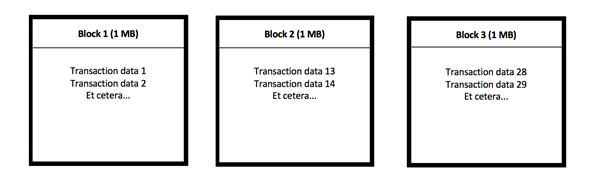
\includegraphics[width=0.8\linewidth,keepaspectratio]{blkchn_1}

{\tiny (Ref:``How does blockchain work in 7 steps — A clear and simple explanation.'' - Jimi S, Good Audience)}
\end{center}

\end{frame}

%%%%%%%%%%%%%%%%%%%%%%%%%%%%%%%%%%%%%%%%%%%%%%%%%%%%%%%%%%%%%%%%%%%%%%%%%%%%%%%%%%
\begin{frame}[fragile]\frametitle{Step 2 — Chaining the blocks (with a hash)}
\begin{itemize}
\item Let’s say block 1 registers two transactions, transaction 1 and transaction 2
\item Assume these fill up 1MB data limit.
\item This block of data now gets a signature for this specific string of data. Let’s say the signature is ‘X32’.
\item Similarly next set of transactions go to Block 2 with a signature '9BZ'.
\item Block 2 gets appended to the existing chain (ie Block 1) 
\item The signatures link the blocks to each other
\end{itemize}

\begin{center}
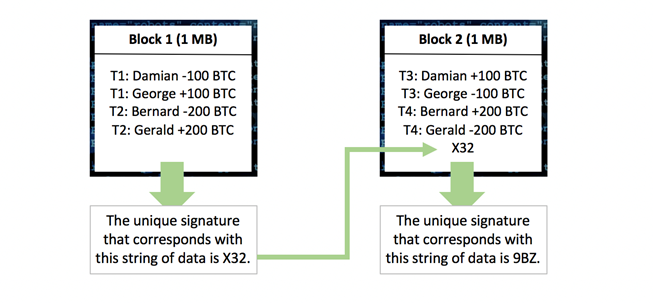
\includegraphics[width=0.6\linewidth,keepaspectratio]{blkchn_2}

{\tiny (Ref:``How does blockchain work in 7 steps — A clear and simple explanation.'' - Jimi S, Good Audience)}
\end{center}

\end{frame}

%%%%%%%%%%%%%%%%%%%%%%%%%%%%%%%%%%%%%%%%%%%%%%%%%%%%%%%%%%%%%%%%%%%%%%%%%%%%%%%%%%
\begin{frame}[fragile]\frametitle{Step 2 — Chaining the blocks (with a hash)}
\begin{itemize}
\item One more block comes (ie Block 3), it gets appended in a similar manner.
\item Now imagine if the data in block 1 is altered.
\item Damian now supposedly sent 500 Bitcoin to George instead of 100 Bitcoin.
\item Block 1's signature now changes, say it is now ‘W10’
\end{itemize}

\begin{center}
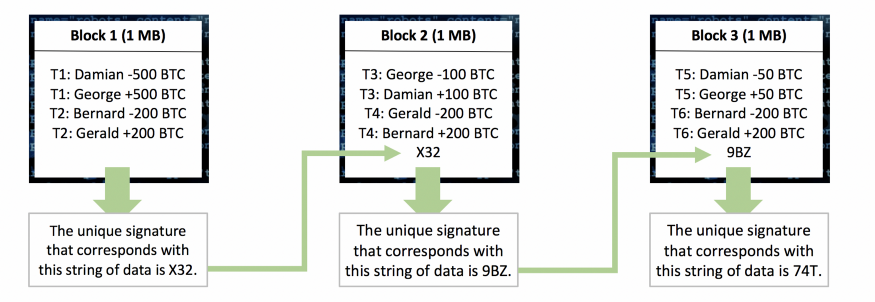
\includegraphics[width=0.6\linewidth,keepaspectratio]{blkchn_3}

{\tiny (Ref:``How does blockchain work in 7 steps — A clear and simple explanation.'' - Jimi S, Good Audience)}
\end{center}

\end{frame}

%%%%%%%%%%%%%%%%%%%%%%%%%%%%%%%%%%%%%%%%%%%%%%%%%%%%%%%%%%%%%%%%%%%%%%%%%%%%%%%%%%
\begin{frame}[fragile]\frametitle{Step 2 — Chaining the blocks (with a hash)}
\begin{itemize}
\item The signature W10 does not match the signature that was previously added to block 2 anymore. 
\item Block 1 and 2 are now considered no longer chained to each other. 
\item Blockchain rejects this change by shifting back to their previous record of the blockchain where all the blocks are still chained together (the record where Damian sent 100 BTC to George).
\item If you try to change pointer in Block 2, its data changes, this signature changes and so on
\item This means that altering a single block requires a new signature for every other block that comes after it all the way to the end of the chain. This is considered to be near impossible.
\end{itemize}

\begin{center}
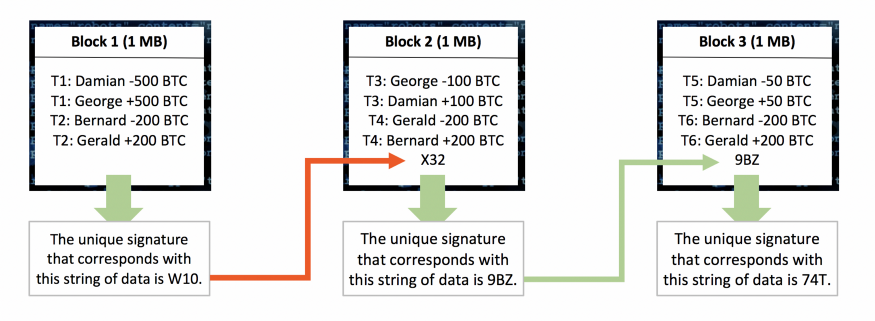
\includegraphics[width=0.6\linewidth,keepaspectratio]{blkchn_4}

{\tiny (Ref:``How does blockchain work in 7 steps — A clear and simple explanation.'' - Jimi S, Good Audience)}
\end{center}

\end{frame}

%%%%%%%%%%%%%%%%%%%%%%%%%%%%%%%%%%%%%%%%%%%%%%%%%%%%%%%%%%%%%%%%%%%%%%%%%%%%%%%%%%
\begin{frame}[fragile]\frametitle{Step 3 — How the signature (hash) is created}
\begin{itemize}
\item Signature is created by a cryptographic hash function. 
\item Takes any string of input and turns it into a unique 64-digit string of output.
\item e.g. ``761A7DD9CAFE34C7CDE6C1270E17F773025A61E511A56F700D415F0D3E199868''
\item If a single digit of the input changes, including a space, changing a capital letter or adding a period for example, the hash will be totally different.
\item But same string 'guarantees' same hash.
\end{itemize}

\begin{center}
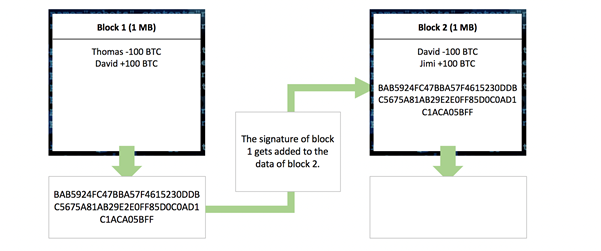
\includegraphics[width=0.6\linewidth,keepaspectratio]{blkchn_5}

{\tiny (Ref:``How does blockchain work in 7 steps — A clear and simple explanation.'' - Jimi S, Good Audience)}
\end{center}

\end{frame}

%%%%%%%%%%%%%%%%%%%%%%%%%%%%%%%%%%%%%%%%%%%%%%%%%%%%%%%%%%%%%%%%%%%%%%%%%%%%%%%%%%
\begin{frame}[fragile]\frametitle{Step 4 — When does the signature qualify, and who signs a block?}
\begin{itemize}
\item A block will only be accepted on the blockchain if its digital signature starts with — for example — a consecutive number of zeroes, Say, 10.
\item String of data of a block needs to be changed repeatedly until that specific string of data leads to a signature starting with ten zeroes. 
\item Because the transaction data and metadata (block number, timestamp, et cetera) need to stay the way they are, a small specific piece of data, called `nonce` is added to every block that has no purpose except for being changed repeatedly in order to find an eligible signature.
\item This is called mining and is what miners do. More compute you have (and luck), faster the process would be.
\end{itemize}

\begin{center}
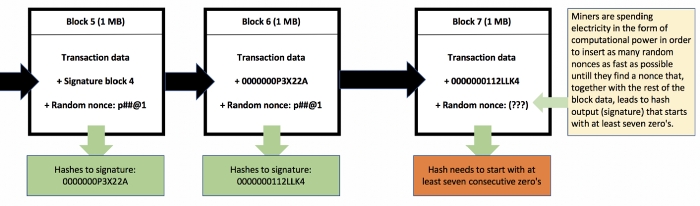
\includegraphics[width=0.6\linewidth,keepaspectratio]{blkchn_6}

{\tiny (Ref:``How does blockchain work in 7 steps — A clear and simple explanation.'' - Jimi S, Good Audience)}
\end{center}

\end{frame}

%%%%%%%%%%%%%%%%%%%%%%%%%%%%%%%%%%%%%%%%%%%%%%%%%%%%%%%%%%%%%%%%%%%%%%%%%%%%%%%%%%
\begin{frame}[fragile]\frametitle{Step 4 — When does the signature qualify, and who signs a block?}
\begin{itemize}
\item Any user on a blockchain network can participate in this process by downloading and starting the according mining software for that specific blockchain. 
\item When a user does this, they will simply put their computational power to work in order to try to solve the nonce for a block.
\item As you can see, the hash (signature) of this block and the hash of the previous block both start with a number of zeroes. 
\end{itemize}

\begin{center}
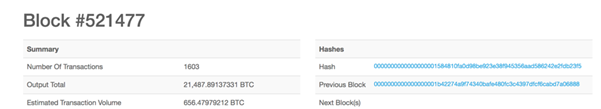
\includegraphics[width=0.6\linewidth,keepaspectratio]{blkchn_7}

{\tiny (Ref:``How does blockchain work in 7 steps — A clear and simple explanation.'' - Jimi S, Good Audience)}
\end{center}

\end{frame}

%%%%%%%%%%%%%%%%%%%%%%%%%%%%%%%%%%%%%%%%%%%%%%%%%%%%%%%%%%%%%%%%%%%%%%%%%%%%%%%%%%
\begin{frame}[fragile]\frametitle{Step 5 — How does this make the blockchain immutable?}
\begin{itemize}
\item Let’s say a corrupt miner has altered a block of transactions and is now trying to calculate new signatures for the subsequent blocks in order to have the rest of the network accept his change. 
\item The problem for him is, the rest of the network is also calculating new signatures for new blocks. 
\item The corrupt miner will have to calculate new signatures for these blocks too as they are being added to the end of the chain.
\item Unless the miner has more computational power than the rest of the network combined, he will never catch up with the rest of the network finding signatures.
\end{itemize}

\begin{center}
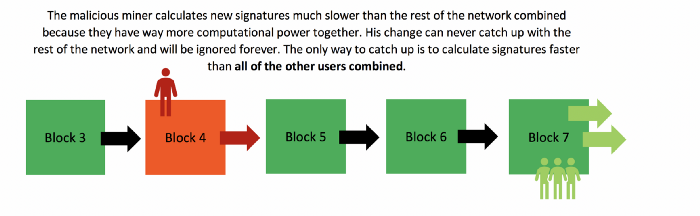
\includegraphics[width=0.6\linewidth,keepaspectratio]{blkchn_8}

{\tiny (Ref:``How does blockchain work in 7 steps — A clear and simple explanation.'' - Jimi S, Good Audience)}
\end{center}

\end{frame}

%%%%%%%%%%%%%%%%%%%%%%%%%%%%%%%%%%%%%%%%%%%%%%%%%%%%%%%%%%%%%%%%%%%%%%%%%%%%%%%%%%
\begin{frame}[fragile]\frametitle{Step 5 — How does this make the blockchain immutable?}
\begin{itemize}
\item What if a bad actor has more computational power than the rest of the network combined? Theoretically yes, this is possible. 
\item It is called a 51\% attack
\item It would not just require an immense amount of hardware, cooling equipment and storage space for the computational power, but also involves the risk of prosecution and, more importantly, would dramatically harm the ecosystem of the corresponding blockchain, rendering the potential returns in Bitcoin to drop significantly in value. 
\item This is also the reason that the more users participate in the mining process, the more secure a blockchain becomes.
\end{itemize}


\end{frame}

%%%%%%%%%%%%%%%%%%%%%%%%%%%%%%%%%%%%%%%%%%%%%%%%%%%%%%%%%%%%%%%%%%%%%%%%%%%%%%%%%%
\begin{frame}[fragile]\frametitle{Step 6 — How is the blockchain governed? Who determines the rules?}
\begin{itemize}
\item A governance model of democracy, so Majority wins.
\item It requires the majority of the computational power to create the longest version of the blockchain. 
\item This is also how an altered block is automatically rejected by the majority of the network.
\item On the Bitcoin blockchain, all transaction history and wallet balances are public (blockchain.info). 
\item Anyone can look up any wallet or transaction that has ever occurred all the way back to the first transaction that was ever made (on January 3rd, 2009). 
\item Although wallet balances can be checked by anyone publicly, the owners of those wallets remain largely unknown.
\end{itemize}


\end{frame}

%%%%%%%%%%%%%%%%%%%%%%%%%%%%%%%%%%%%%%%%%%%%%%%%%%%%%%%%%%%%%%%%%%%%%%%%%%%%%%%%%%
\begin{frame}[fragile]\frametitle{Final step, step 7 — Where does this leave cryptocurrencies?}
\begin{itemize}
\item Most cryptocurrencies are built upon their own blockchain protocol that may have different rules from the Bitcoin blockchain. 
\item Cryptocurrencies can however be given any kind of value, depending on their issuer. They could be referred to as ‘tokens’. 
\item Any sort of value can be attached to a ‘cryptocurrency’ token. 
\item All these cryptocurrency transactions are registered on various blockchains and can be exchanged online through cryptocurrency exchanges such as Binance. 
\end{itemize}


\end{frame}

